\documentclass[11pt]{article}
\centerline{Daniel E.~Otero}
\centerline{Department of Mathematics}
\centerline{Xavier University}
\centerline{Cincinnati, OH, 45207-4441}
\centerline{\texttt{otero@xavier.edu}}

Students of the differential calculus learn that the fundamental notion of the derivative of a function depends on evaluating this limit: $$f'(a)=\lim_{x\to a} \frac{f(x)-f(a)}{x-a}.$$One's success in obtaining the limit is not at all obvious, since in the quotient that appears here, both the numerator and denominator approach $0$, leaving us to puzzle over what to make of the indeterminate value ${\displaystyle \frac00}$. However, this is a momentary setback; we are soon shown clever algebraic techniques for surmounting this ${\displaystyle \frac00}$ problem. These algebraic manipulations allow us to develop the familiar differentiation rules for many of the functions that turn up in standard applications of calculus in the natural and social sciences.

What may be more surprising to learn is that one of the early successes of the calculus was the discovery of a result that allowed the evaluation of limits of precisely this ${\displaystyle \frac00}$ indeterminate form, and which depended for its success on the calculation of derivatives! This result was announced in the very first comprehensive book-length treatment of the differential calculus in 1696. It is named L'H\^opital's Rule, after the author of this same book, so its historical pedigree is deep, and is further reflected in that nearly every first-semester calculus student still learns L'H\^opital's Rule today, more than 300 years later, as the chief method for evaluating limits of indeterminate type.

In this project, we will first examine limits of indeterminate type ${\displaystyle \frac00}$ as they might appear in a natural setting. Then, we will read from L'H\^opital's early calculus book about how differential calculus was understood then as a literal calculus of differentials, well before the notion of a function's derivative was formulated. We will then see how differentials were employed to justify this eponymous Rule. Finally, we will see how to apply the Rule to evaluate some limits of indeterminate type.


\newpage
\section{Limits of Indeterminate Type}

Let's set the stage with an exploration of the behavior of certain kinds of rational functions\footnote{Recall that, by analogy with rational numbers, a rational function $r(x)$ is one that is defined as a quotient $\frac{p(x)}{q(x)}$ of two polynomials $p(x)$ and $q(x)$.}:

\begin{task}[\label{factorable}]
\begin{enumerate}[(a)] \itemsep -8pt
\item Use a graphing utility to produce a graph of the rational function $$r(x)=\frac{x^3+3x-4}{x-1}$$over the interval $-2 \le x \le 2$. What sort of curve is this? \\
\item Now graph the function $s(x)=x^2+x+4$ over the same interval $-2 \le x \le 2$, and compare it with part (a). Describe the relationship between the functions $r(x)$ and $s(x)$ that is borne out in their graphs. \\
\item Build a five-column table of values like the one below, in which the first column lists the inputs $x=-2, -1, 0, 1, 2$, while the second, third and fourth columns list the corresponding outputs for the numerator polynomial $p(x)=x^3+3x-4$, the denominator polynomial $q(x)=x-1$, and their quotient, the rational function $r(x)$. %(For reasons that should become clear, it is strongly advised that you record the values of $r(x)$ as \emph{fractions}, not decimals.) 
In the fifth column, supply the outputs for the function $s(x)$. 

\begin{center}
\begin{tabularx}{0.75\textwidth}{c|CCC|C}
$x$ & $p(x)$ & $q(x)$ & $r(x)$ & $s(x)$ \\ \hline
$-2$ &&&& \\
$-1$ &&&& \\
$\vdots$ &&&&
\end{tabularx}
\end{center}
\bigskip

\item[] How does this information shed light on the relationship between $r(x)$ and $s(x)$? \\
\item Now try factoring the polynomial $p(x)$. How does this help explain the relationship between $r(x)$ and $s(x)$? \\
\item More generally (that is, for every possible value of $x$), how do the values of the functions $r(x)$ and $s(x)$ differ? \\
\item Use a graphing utility to produce a graph of the rational function $$t(x)=\frac{x^3+3x^2-4}{x-1}$$over the interval $-4 \le x \le 4$. (\emph{Note the slight difference between the formulas for $t(x)$ and $r(x)$}.) Describe as best you can the differences between the graphs of $t(x)$ and $r(x)$.
\end{enumerate}
\end{task}

\newpage
%\bigskip
\begin{task}[\label{not_so_easy}]
\begin{enumerate}[(a)] \itemsep -8pt
\item As in Task 1, use a graphing utility to produce a graph of the rational function $$R(x)=\frac{x^4-6x^2+1}{x^2-2x-1}$$over the interval $-4 \le x \le 4$. What sort of curve is this? How can you tell? \\
\item It's far more difficult to factor the numerator polynomial $P(x)=x^4-6x^2+1$ (and the denominator polynomial $Q(x)=x^2-2x-1$ for that matter) than in the example in Task 1. Nonetheless, can you still find a quadratic function $S(x)$ that agrees with $R(x)$ at every point where $R(x)$ is defined? Describe your thinking about this problem. \\
\item Now produce a graph of the rational function $$T(x)=\frac{x^4-6x^2-1}{x^2-2x-1}$$ over the interval $-4 \le x \le 4$. (Again, note the slight difference between the formulas for $T(x)$ and $R(x)$.) Describe as best you can the differences between the graphs of $T(x)$ and $R(x)$.
\end{enumerate}
\end{task}

\bigskip
\begin{task}[\label{exponential_numerator}]
\begin{enumerate}[(a)] \itemsep -8pt
\item Use a graphing utility to produce a graph of the two functions $$w(x)=\frac{2^x-1}{2x}\quad\textrm{ and }\quad W(x)=\frac{2^x+1}{2x}$$over the interval $-4 \le x \le 4$. What can you say about the $y$-intercepts of these two functions? \\
\item The numerator functions $u(x)=2^x-1$ and $U(x)=2^x+1$ are not polynomials (even though the common denominator function $v(x)=V(x)=2x$ is). So $w(x)$ and $W(x)$ are \emph{not} rational functions. Describe how this difference prevents us from analyzing the behavior of the functions $w(x)$ and $W(x)$ in the same way that we dealt with $r(x)$ and $R(x)$ in the previous two tasks. \\
\item You may have recognized that $w(0)$ and $W(0)$ are undefined, but your graphs of these functions may make it hard to tell. Indeed, the graph indicates that $w(x)$ is perfectly well defined at every other value of $x$ besides $x=0$, and that $$\lim_{x\rightarrow 0} w(x)$$ is also well defined! Numerically determine the value of this limit to four decimal place accuracy by computing values of $w(x)$ for at least five increasingly smaller positive values of $w(x)$ and at least five increasingly larger negative values of $w(x)$.
\end{enumerate}
\end{task}

\newpage
%\bigskip
\begin{task}[\label{continuity}]
\begin{enumerate}[(a)] \itemsep -8pt
\item Is the function $r(x)$ from Task \ref{factorable} continuous everywhere? Is the function $R(x)$ from Task \ref{not_so_easy} continuous everywhere? How about $w(x)$ from Task \ref{exponential_numerator}? In each case, explain how you know that the particular function is continuous at every real number, or how it fails to meet the criteria for being continuous at certain points. \\
\item Given your results in Tasks \ref{factorable}, \ref{not_so_easy} and \ref{exponential_numerator}, what common properties can you identify about the behavior of the three functions $r(x)$, $R(x)$ and $w(x)$ at the given input values?
\end{enumerate}
\end{task}

\bigskip
If you successfully completed the tasks above, you probably noticed that they illustrate a particular phenomenon in which a given function is undefined at a particular input value $x=a$, despite appearing to be otherwise well-behaved, in the sense that at every other input value the function is both continuous and smooth\footnote{This term ``smooth'' is not often included in the standard terminology of a calculus student, so here's a definition: a function is \emph{smooth} at a particular input value if it and its derivatives, to arbitrarily high order, are well defined there. In particular, all polynomial, exponential and trigonometric functions are smooth at every point where the functions are defined.}! Moreover, the function is ``as close as possible'' to being continuous at the relevant point since the \emph{limiting value} of the function exists there even though the \emph{function value} does not.

Recall that a function $f$ of a real variable $x$ is \emph{continuous at a point} $x=a$ provided three conditions hold:
\begin{enumerate} \itemsep -3pt
\item the function is defined there, that is, $f(a)$ exists;
\item the limiting value of the function is defined there, that is, ${\displaystyle\lim_{x\rightarrow a} f(x)}$ exists;
\item and the two values agree: ${\displaystyle\lim_{x\rightarrow a} f(x)=f(a).}$
\end{enumerate}
Most functions that are studied in calculus courses are continuous at all points where they are defined. Indeed, we often depend on this to help us evaluate the limit computations we encounter: often, our first inclination on needing to determine a limit ${\displaystyle \lim_{x\rightarrow a} f(x)}$ is to rely on the continuity of the function $f$ by simply evaluating $f(a)$.

But in the situations described in the Tasks above, the functions $r(x)$ and $R(x)$ turn out to be discontinuous at $x=1$, and $w(x)$ is discontinuous at $x=0$, all because the given functions are \emph{undefined} at the relevant point, making it impossible to use this method to determine the limiting values. Moreover, the three functions were discontinuous \emph{in the same way}: each is the quotient of a numerator and denominator function that vanishes at the particular input value, meaning that an attempt to evaluate the function at this input leads to the value $\frac00$, a meaningless and undefined quantity.

If $u(x)$ and $v(x)$ are a pair of functions that satisfy ${\displaystyle \lim_{x\to a}} u(x)=0$ and ${\displaystyle \lim_{x\to a}} v(x)=0$, then we call 
\begin{equation}\label{indeterminate}
\lim_{x\to a} \frac{u(x)}{v(x)}
\end{equation}
 a {\bf limit of indeterminate type $\frac00$}.

Now in the case of $r(x)$ and $R(x)$ in the Tasks above, even though we were presented with a limit of indeterminate type, we found a way to determine it because the numerator and denominator functions were polynomials with a common factor, a factor which was entirely responsible for the vanishing of the numerator and denominator. We were able to divide out the offending factor and thereby resolve the limit. 

But this was not the case in Task \ref{exponential_numerator}; the best we could do there was to approximate the desired limit. Ah, never fear! This is a job for \dots calculus! Indeed, as we shall discover below, resolving the problem of limits of indeterminate type was among the first of many successful applications of the new calculus techniques that were developed in the late seventeenth century.
\bigskip
%\newpage

\section{L'H\^opital's \emph{Analyse} and the Calculus of Differentials}
%\value{\tasknumb}


What we call calculus today was first formulated as a body of related mathematical techniques by two men working independently in the late 1600s: Isaac Newton (1642--1727) in Britain, and Gottfried Leibniz (1646--1716) on the European Continent. Leibniz discovered simple symbolic computational techniques, a ``calculus''\footnote{The word \emph{calculus} is Latin for ``pebble'', describing the token that was used on ancient counting boards as an aid for doing arithmetic in the times before modern mechanical or electronic computers. Leibniz used the word to refer to the new calculation methods he had discovered.}  as he called it, that led to the development of a systematic mathematical theory for the motion of physical objects. Newton's success in using these ideas to explain the celestial motions of the planets in their elliptical orbits, and at the same time, how falling bodies behaved here on earth\footnote{Newton published his wildly popular \emph{Philosophiae Naturalis Principia Mathematica} (\emph{Mathematical Principles of Natural Philosophy}) in 1687, but did so without acknowledging the new concepts of his calculus due to his extreme reluctance to divulge any methods. His calculus would later be published posthumously, in \emph{The Method of Fluxions} (1736).}, turned the heads of mathematicians and scientists across Europe at the dawn of the eighteenth century. Scientists would spend the next 400 years extending the reach of application of the ideas first formulated by these two men, building the mathematical tools fundamental to the development of astronomy, physics, chemistry, biology, engineering sciences, and eventually computer science, thereby ushering in the modern age of technology, a movement still playing out in our times.

%Among the first scientists to contribute to this development were contemporaries of Newton and Leibniz: a French nobleman, Guillaume Fran\c{c}ois Antoine, Marquis de l'H\^opital (1661--1704); and a Swiss-born mathematician, Johann Bernoulli (1667--1748). As a young aristocrat in his twenties, L'H\^opital had to abandon a career in the military because of his severe nearsightedness, but he was passionate about mathematics, so he attached himself to a circle of mathematicians in Paris, where the new analytic theories of Newton and Leibniz were being discussed and studied. There, in 1691, L'H\^opital made the acquaintance of Bernoulli, discovering that the younger man had a much stronger command of these ideas than did he. Bernoulli, the tenth of his parents' children, was something of a disappointment to his father who expected him to take up a profitable career in business. Johann managed to convince him to allow him to enroll at the university in his native Basel, however, where he followed a path laid down by his brother Jakob, 12 years his elder, who had similarly deflected their father's desire for him to study theology, taking up mathematics instead. In the 1680s, the two young Swiss mathematicians became experts in the new calculus espoused by Leibniz, with whom they communicated through letters and in the pages of new academic journals that were being published. Eventually, both would have the chair of Mathematics at the University of Basel, Johann succeeding Jakob there in 1705 after the death of his elder brother.

Among the first scientists to contribute to this development were three contemporaries of Newton and Leibniz: a pair of Swiss-born mathematicians, Jakob Bernoulli (1655--1705) and his younger brother Johann Bernoulli (1667--1748), and a French nobleman, Guillaume Fran\c{c}ois Antoine, Marquis de l'H\^opital (1661--1704). Jakob, the older brother, successfully deflected his father's desire for him to study theology at the University of Basel, taking up mathematics instead. His younger brother Johann was another disappointment to his father, as he was expected him to take up the profitable family business but was drawn into the exciting new world of mathematics to which Jakob introduced him.  In the 1680s, the two brothers became experts in the new calculus espoused by Leibniz, with whom they communicated through letters and in the pages of new academic journals that were being published. Eventually, both would hold the chair of Mathematics at the University of Basel, Johann succeeding Jakob there in 1705 after the death of his elder brother.

As a young aristocrat in his twenties, the Marquis de L'H\^opital had to abandon a career in the military due to severe nearsightedness. But he was passionate about mathematics, so he attached himself to a circle of mathematicians in Paris, where the new analytic theories of Newton and Leibniz were being discussed and studied. There, in 1691, L'H\^opital made the acquaintance of Jophann Bernoulli, discovering that the younger man had a much stronger command of these ideas than did he. Soon after they met, L'H\^opital, anxious to learn what he could of the new mathematical theories, engaged Johann to give him private lectures on the calculus, both in Paris and at the nobleman's estate in Oucqes just outside the city, and he provided Johann with handsome compensation for his pains. This arrangement ultimately led to the publication by L'H\^opital of the first comprehensive treatment of the subject of the differential calculus, \emph{Analyse des infiniment petits pour l'intelligence des lignes courbes} [\emph{Analysis of the infinitely small, for the understanding of curved lines}] in 1696 (and then in a posthumous second edition in 1715) \citep{LHopital}.\footnote{The book has recently been released in a modern English translation \citep{Bradley}, from which the excerpts found in these pages have been drawn.} It is in L'H\^opital's \emph{Analyse} that we find the very first application of the subject to the resolution of limits of indeterminate type!

Leibniz' version of the calculus began as a theory not about derivatives, in the way that we learn the subject today, but about \emph{differentials}. We see this in the way that L'H\^opital sets out his (that is, Bernoulli's) understanding of calculus in the opening chapter of the \emph{Analyse}.

\bigskip
\vspace*{-5pt}
\begin{source}
{\bf Chapter 1. In Which We Give the Rules of This Calculus}

%[\dots]

\begin{center}
	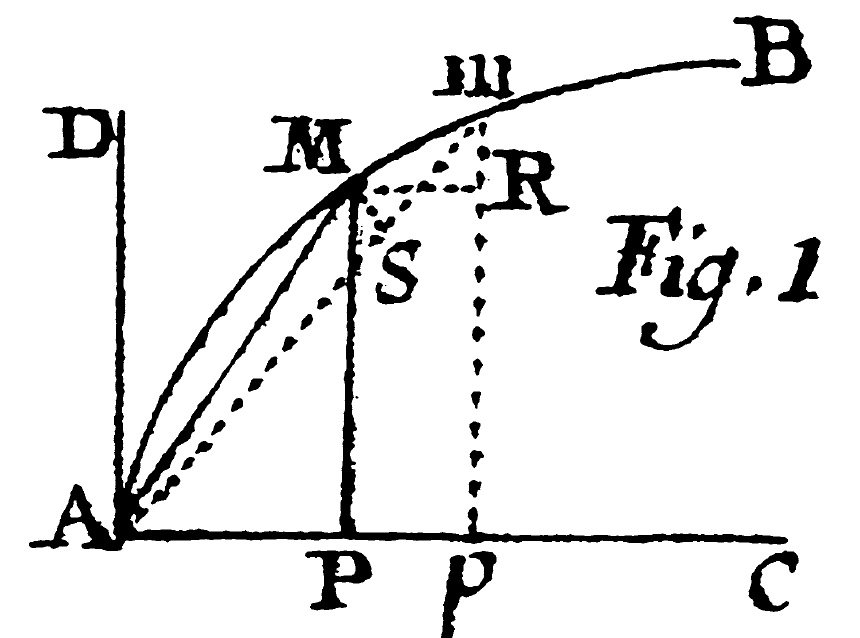
\includegraphics[width=6cm]{LH_Fig1.jpeg}
\end{center}

{\bf Definition.} The infinitely small portion by which a variable quantity continually increases or decreases is called the \emph{Differential}. For example, let $AMB$ be an arbitrary curved line (Fig.~1) which has the line $AC$ as its axis or diameter, and has $PM$ as one of its ordinates.\footnote{In L'H\^opital's day, mathematicians preferred the classical terms \emph{abscissa} and \emph{ordinate} for what we today call respectively the $x$- and $y$-coordinates of a point.} Let $pm$ be another ordinate, infinitely close to the first one. Given this, if we also draw $MR$ parallel to $AC$, and the chords $AM\; Am$, and describe the little circular arc $MS$ of the circle with center $A$ and radius $AM$, then $Pp$ is the differential of the $AP$, $Rm$ the differential of $PM$, $Sm$ the differential of $AM$, and $Mm$ the differential of the arc $AM$. Furthermore, the little triangle $MAm$, which has the arc $Mm$ as its base is the differential of the segment $AM$, and the little region $MPpm$ is the differential of the region contained by the straight lines $AP$ and $PM$, and by the arc $AM$. [\dots]

\emph{Note.} In what follows, we will make use of the symbol $d$ to denote the differential of a variable quantity that is expressed by a single letter and, in order to avoid confusion, the letter $d$ will not be used in any other way in the following calculations. If, for example, we denote $AP$ by $x$, $PM$ by $y$, $AM$ by $z$, the arc $AM$ by $u$, the curvilinear region $APM$ by $s$, and the segment $AM$ by $t$, then $dx$ denotes the value of $Pp$, $dy$ that of $Rm$, $dz$ that of $Sm$, $du$ that of the little arc $Mm$, $ds$ that of the little region $MPpm$, and $dt$ that of the little curvilinear triangle $MAm$.
\end{source} \label{Ch1}
\newpage

\bigskip

%\setcounter{tasknumb}{4}
\begin{task}[\label{Differential}]
\begin{enumerate} \itemsep -10pt
\item[(a)] What do you think L'H\^opital meant by ``infinitely small''? Is it the same as having no size? For instance, in Fig.~1, even though $pm$ is meant to be drawn ``infinitely close'' to $PM$, there is clearly a measurable gap between them. How big is the corresponding differential $Pp$ (later called $dx$) supposed to be? Are $P$ and $p$ different points? Share your thoughts about these questions. \\
\item[(b)] Sketch for yourself a larger version of L'H\^opital's Figure 1 complete with the labeled points $A, B, C, D, M, m, P, p, R, S$. (You can omit the notation for ``Fig.~1''.) Then attach labels for the various differentials $dx, du, ds$ and $dt$ to the proper element for each in the diagram. \\
\item[(c)] In what ways are these differential quantities geometrically similar?
\end{enumerate}
\end{task}
\vspace{-0.25in}

\begin{source}

%{\bf Postulate I.} (\S2) We suppose that two quantities that differ by an infinitely small quantity may be used interchangeably, or (what amounts to the same thing) that a quantity which is increased or decreased by another quantity that is infinitely smaller that it is, may be considered as remaining the same. We suppose, for example, that we may take $Ap$ for $AP$, $pm$ for $PM$, the region $Apm$ for $APM$, the little region $MPpm$ for the little rectangle $MPpR$, the little sector $AMm$ for the little triangle $AMS$, the angle $pAm$ for the angel $PAM$, and so forth.

{\bf Postulate.} %II.} (\S3)
We suppose that a curved line may be considered as an assemblage of infinitely many straight lines, each one being infinitely small, or (what amounts to the same thing) as a polygon with an infinite number of sides, each being infinitely small, which determine the curvature of the line by the angles formed amongst themselves. We suppose, for example, that the portion $Mm$ of the curve %and the arc $MS$ of the circle 
\dots may be considered to be straight lines on account of their infinite smallness. \dots%, so that the little triangle $mSM$ may be considered to be rectilinear.

\bigskip

{\bf Chapter 2. Use of the Differential Calculus for Finding the Tangents of All Kinds of Curved Lines}

\begin{center}
	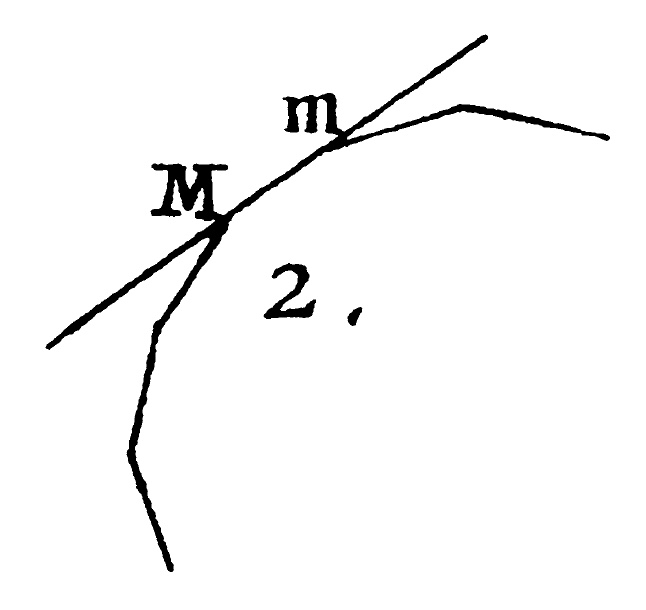
\includegraphics[width=4.25cm]{LH_Fig2.jpeg}
\end{center}
\vspace{-0.1in}

{\bf Definition.} If we prolong one of the little sides $Mm$ (Fig.~2) of the polygon that makes up a curved line, this little side, thus prolonged is called the Tangent to the curve at the point $M$ or $m$.

\begin{center}
	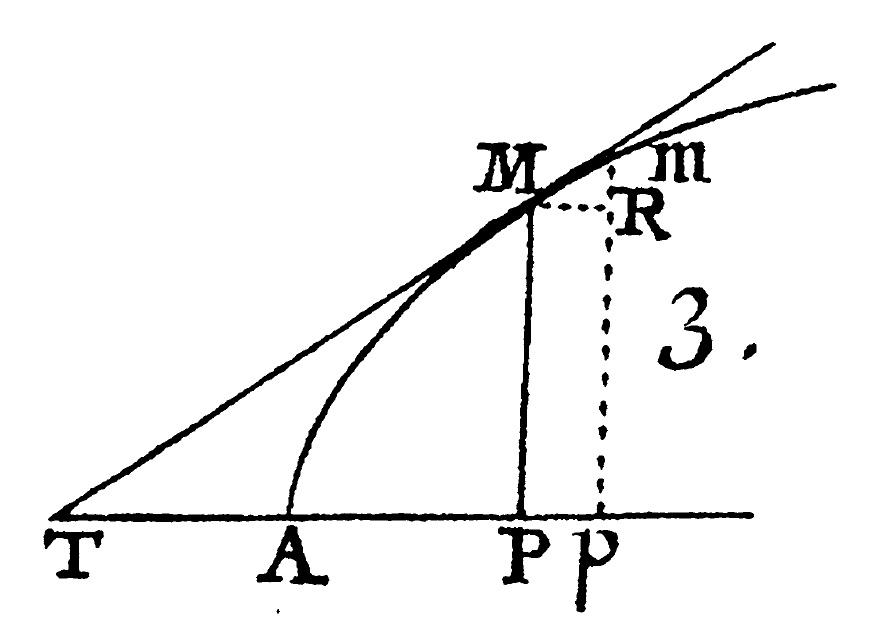
\includegraphics[width=5.75cm]{LH_Fig3.jpeg}
\end{center}
\vspace{-0.1in}
\end{source}

\newpage
\begin{task}[\label{Tangents}]
The curve $AM$ in Figure 3 at the end of the last excerpt\footnote{This figure is reproduced again at the bottom of this page.} could be a sketch of the graph of the function $y=\sqrt{x}$, where $A$ is the origin of the coordinate system and $M$ and $m$ are other points on this parabolic curve. (We know that the curve is a parabola since it is a portion of the graph of the equation $x=y^2$.)
\begin{enumerate}
\item[(a)] Let's take $M=(\frac14, \frac12)$ on this portion the curve. Use your knowledge of calculus to determine the equation of the tangent line $MT$ to this curve at $M$. \\
\item[(b)] If $M$ and $m$ are the same two points displayed in the ``close-up'' of Figure 2, how close together are these points meant to be? \\
\item[(c)] In Figure 2, the ``little side'' $Mm$ lies to the right of $M$; let $m'$ denote the other endpoint of the ``little side'' to the left of $M$ so that $m'M$ is the adjacent side to $Mm$ of the ``polygon with an infinite number of sides'' that makes up the curve. How close together are $M$ and $m'$? \\
\item[(d)] If the ``prolongation'' of $Mm$ produces the tangent line to the curve at $M$ containing the point $T$, does the ``prolongation'' of $m'M$ also produce a tangent line to the curve at $M$? How many tangent lines are there to the curve at $M$? On a related note, what is the measure of the angle $m'Mm$? Can you bring some clarity to an understanding of these diagrams?
\end{enumerate}
\end{task}


%\bigskip
Perhaps Task \ref{Tangents} %%. !!!!!!!!!!???????
has seeded doubt in your mind that L'H\^opital and Bernoulli (and Leibniz, who they were following) had any idea what they were doing, basing their understanding of calculus on such problematic notions as the ``infinitely small''. If we read on, however, it will become clear that they really did have the basic ideas right.

\bigskip

\begin{source}

\begin{center}
	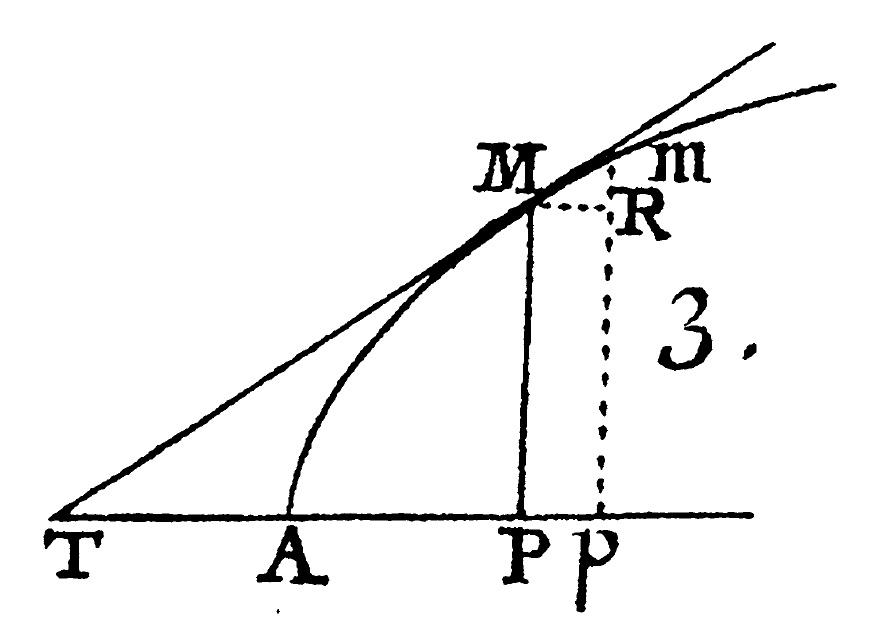
\includegraphics[width=5.75cm]{LH_Fig3.jpeg}
\end{center}

{\bf Proposition I.}

{\bf Problem.} (\S9) Let $AM$  be a curved line (Fig.~3) where the relationship between the abscissa $AP$ and the ordinate $PM$ is expressed by any equation. At a given point $M$ on this curve, we wish to draw the tangent $MT$.\footnote{It is worth noting that L'H\^opital wrote this before the notion of the slope of a line was developed. He and his contemporaries were genuinely interested in the geometric problem of \emph{drawing} the tangent to the curve at the point, and his goal here is to find a method for doing this.}

\renewcommand*{\thefootnote}{\fnsymbol{footnote}}

We draw the ordinate $MP$ and suppose that the straight line $MR$ that meets the diameter at the point $T$ is the tangent we wish to find. We imagine another ordinate $mp$ infinitely close to the first one, with a little straight line $MR$ parallel to $AP$. Now denoting the given quantities $AP$ by $x$ and $PM$ by $y$ (so that $Pp$ or $MR=dx$ and $Rm=dy$), the similar triangles $mRM$ and $MPT$ give\footnote[1]{Translator's Footnote: {\sf In \citep{LHopital} the notation $a\, .\, b :: c\, .\, d$ was used to express equal proportion; we write this instead as $a : b :: c : d$. We note further that in \citep{LHopital} the right parenthesis following $dx$ was omitted.}} $mR(dy) : RM(dx) :: MP(y) : PT=\frac{ydx}{dy}$. Now, by means of the differential of the given equation, we find a value for $dx$ in terms that are multiplied by $dy$. This (being multiplied by $y$ and divided by $dy$) will give the value of the subtangent $PT$ in terms that are entirely known and free of differentials, which can be used to draw the tangent that we wish to find.
\end{source}

\smallskip
\begin{task}[\label{find_tangent}]
\begin{enumerate} \itemsep -5pt
\item[(a)] Explain why the triangles $mRM$ and $MPT$ are similar, to justify the proportion $mR : RM :: MP : PT$. \\
\item[(b)] Substitute differentials for the first three of the four magnitudes in the proportion above, expressing the proportion as an equation of fractions, to conclude, as indicated by L'H\^opital, that $PT=\frac{ydx}{dy}$. \\
\item[(c)] Rewrite the last equation in the form $PT=\frac{y}{(dy/dx)}$, then use the calculus you're familiar with to find the derivative of $y=\sqrt{x}$, and substitute it into this formula. As a result, determine a formula for $PT$ in terms of $x$. \\
\item[(d)] Finally, use the fact that we chose $M=(\frac14, \frac12)$ to determine the coordinates of $T$ from your result in part (c). Do you get the same answer as the $x$-intercept of the tangent line you found in Task \ref{Tangents}(a)?
\end{enumerate}

 \end{task}

\smallskip
From the time of the ancient Greeks, geometers knew how to draw the tangent to a parabola at any point on the curve, so this problem outlined in L'H\^opital's \emph{Analyse} was not a discovery made possible by the invention of calculus but rather a confirmation of the power of the newer techniques. Further proof of the power of calculus came from its ability to extend geometers' ability to deal with other kinds of curves besides the traditional parabola.

\smallskip
\begin{source}
Let the general equation be $y^m=x$, which expresses the nature of all parabolas to infinity, when the exponent $m$ denotes a whole or fractional positive number, and of all hyperbolas when it denotes a negative number. Taking differentials, we have $my^{m-1}\,dy=dx$ and thus $PT\,\left([\textrm{or}] \frac{y\,dx}{dy}\right)=my^m=mx$, substituting the value $x$ for $y^m$.
\end{source}

\bigskip
\begin{task}[\label{traditional_parabola}]
Verify that setting $m=2$ in the paragraph above leads to the case of the traditional parabola, which L'H\^opital worked out in his Proposition I.
 \end{task}

\bigskip
In the previous source excerpt, L'H\^opital calls the procedure that takes the equation of the ``general parabola'' $y^m=x$ and produces from it the equation $my^{m-1}dy=dx$ ``taking differentials''. It is important to note that in the early years of calculus, the fundamental idea was not the derivative, but the differential. It was only about 100 years later, after they grew comfortable using the ideas of Leibniz's calculus, that mathematicians realized that the most powerful manifestation of differentials was in determining their ratios, and that a more convenient way to organize calculus was not in terms of relations between differentials, as in the equation $my^{m-1}dy=dx$, but rather to focus on the properties of their ratios, as in the equivalent equation 
\begin{equation}\label{general_parabola_derivative}
\frac{dy}{dx}=\frac{1}{m}x^{(1-m)/m}.
\end{equation}
When Joseph-Louis Lagrange (1736--1813) wrote up lecture notes for his calculus students at the \`Ecole Polytechnique in Paris in the 1790s \citep{Lagrange}, his reformulation of the theory introduced the \emph{derivative} of a function $y=f(x)$, which he denoted $y'=f'(x)$, as the ratio of the differentials $\frac{dy}{dx}$. This began a shift in the standard treatment of the subject in which derivatives of functions superseded the differentials of quantities as the main focus of attention in calculus.

\bigskip
\begin{task}[\label{general_parabola}]
Solve $y^m=x$ for $y$, then compute the derivative to verify equation (\ref{general_parabola_derivative}).
 \end{task}

\bigskip
\begin{task}[\label{cubical_parabola}]
Suppose that Figure 3 now displays (the upper part of) the graph of a \emph{cubical parabola} $y^3=x$. If $M$ is the point with coordinates $(8,2)$, use L'H\^opital's result in the last excerpt above to determine the coordinates of the point $T$. Use a graphing utility to produce a graph of this curve and the tangent line at the point $M$.
 \end{task}

\bigskip
\section{L'H\^opital's Rule: Determining Limits of Indeterminate Type} 

Chapter 2 of L'H\^opital's \emph{Analyse} is a presentation of Leibniz's theory of differentials as told by Bernoulli and organized by L'H\^opital. The next chapters of the book apply these ideas to the study of the properties of a variety of curves%, many of which were long part of the lexicon of geometers since the time of the ancient Greeks
. Then in Chapter 9, attention is turned to the problem of limits of indeterminate type.


 \bigskip
\newpage 
\begin{source}
{\bf Chapter 9. The Solution of Several Problems That Depend upon the Previous Methods}

\begin{center}
	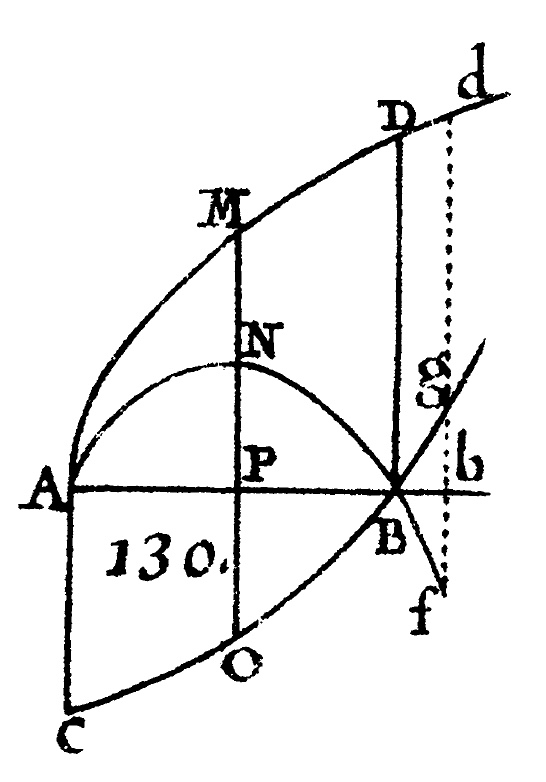
\includegraphics[width=6cm]{LH_Fig130.jpeg}
\end{center}

{\bf Proposition I.}

{\bf Problem.} (\S163) \emph{Let $AMD$ (Fig.~130) be a curved line ($AP=x, PM=y$, and $AB=a$) such that the value of the ordinate $y$ is expressed by a fraction, in which the numerator and the denominator each becomes zero when $x=a$, that is to say, when the point $P$ falls on the given point $B$. We ask what the value of the ordinate $BD$  ought to be.}

Let it be understood that there are two curved lines $ANB$ and $COB$ that have the line $AB$ as a common axis, and which are such that the ordinate $PN$ expresses the numerator, and the ordinate $PO$ the denominator of the general fraction that corresponds to all of the ordinates $PM$, so that $PM=\frac{AB \times PN}{PO}$. It is clear that these two curves meet at the point $B$ because, by the assumption, $PN$ and $PO$ each becomes zero when the point $P$ falls on $B$. 

\end{source}

\bigskip
To assist us in discussing L'H\^opital's Proposition I, let's introduce some other symbols for reference purposes: let $u$ represent the ordinate $PN$ in Fig.~130 in the source above, and let $v$ denote the ordinate $PO$. For simplicity, we further assume that $AB$ has a certain length, i.e., $AB=a$. 

\bigskip
\begin{task}[\label{the_Rule}]
Given this additional notation, explain the connection between the Problem that L'H\^opital presents here and the concept of a limit of indeterminate type $\frac00$ which was defined in equation (\ref{indeterminate}) back in Section 1 of this project.
 \end{task}

\bigskip
L'H\^opital and Bernoulli use differentials to solve the problem of limits of indeterminate type $\frac00$. The following excerpt immediately follows the previous one in L'H\^opital's \emph{Analyse}.
 
\bigskip
\begin{source}

Given this, if we imagine an ordinate $bd$ infinitely close to $BD$, which meets the curved lines $ANB$ and $COB$ at $f$ and $g$ [respectively], then we will have $bd=\frac{AB \times bf}{bg}$, which (see \S2) does not differ from $BD$. It is therefore only a question of finding the ratio of $bg$ to $bf$. Now, it is clear that as the abscissa $AP$ becomes $AB$, the ordinates $PN$ and $PO$ become null, and that as $AP$ becomes $Ab$, they become $bf$ and $bg$. From this, it follows that these ordinate themselves, $bf$ and $bg$, are the differentials of the ordinates at $B$ and $b$ with respect to the curves $ANB$ and $COB$. Consequently, if we take the differential of the numerator and we divide it by the differential of the denominator, after having let $x=a=Ab$ or $AB$, we will have the value that we wish to find for the ordinate $bd$ or $BD$. This is what we were required to find.

\end{source}

\begin{task}[\label{uv}]
Since we have set $u=PN$ and $v=PO$ in Fig.~130, which quantities in the excerpt above correspond to the differentials $du$ and $dv$?
\end{task}

\begin{task}[\label{updated}]
According to L'H\^opital, what exactly is the thing he refers to that ``we were required to find''? Fill in the missing blanks below to express it in terms of $x, y, u$ and $v$.
\begin{quote}
\begin{thm*}[{\bf Proposition I, Updated using Limits}]
Let $u$ and $v$ be ordinates of curves measured against an axis whose abscissa is called $x$; further, suppose that $u$ and $v$ both approach \makebox[0.5in]{\hrulefill} when $x$ approaches \makebox[0.5in]{\hrulefill}. Then (despite the fact that $y=\makebox[0.5in]{\hrulefill}/\makebox[0.5in]{\hrulefill}$ is undefined when $x=$ \makebox[0.5in]{\hrulefill}), the limiting value of $y$ as $x$ approaches \makebox[0.5in]{\hrulefill} (a limit of indeterminate type ${\displaystyle \frac00}$) satisfies
	\begin{equation}\label{OldRule}
	\lim_{x\to a} \frac{u}{v}=\lim_{x\to a} \makebox[0.5in]{\hrulefill}\;.
	\end{equation}
\end{thm*}
\end{quote}
\end{task}

\bigskip
A natural question to ask might be, ``Why didn't L'H\^opital make use of the language of limits to state his proposition, as we did above?'' This question has an easy answer: the concept of a limit hadn't yet been formulated in L'H\^opital's day! Nor would it happen for more than 100 years after L'H\^opital and Bernoulli worked on these problems. Limits were introduced as a way to clarify these central ideas by Augustin-Louis Cauchy (1789--1857) in lecture notes for the course he taught to young engineers at the \'Ecole Polytechnique in Paris in the 1820s.

\begin{task}
Reread the statement of L'H\^opital's Problem at the beginning of his Chapter 9. When he asks ``what the value of the ordinate $BD$ ought to be,'' how might we formulate this question in modern mathematical language?
\end{task}

\bigskip
When we learn about differentials in a presentation of calculus today, they are usually introduced in terms of functions, since today's calculus is founded on the analysis of functions. If $y=f(x)$ is a (differentiable) function of $x$, we interpret the differential $dx$ of the independent variable essentially as Leibniz, Bernoulli and L'H\^opital did, as an infinitely small change in $x$, and then define the differential of $y$ in terms of $dx$ as
\begin{equation} \label{eqn4}
dy=f'(x)\,dx,
\end{equation}
reflecting precisely how $y$ must change \emph{with respect to} $x$.

This reformulation of the differential in terms of derivatives allows us to replace the differentials $du$ and $dv$ in equation (\ref{OldRule}) with expressions involving derivatives instead. In particular, since $$\frac{du}{dv}=\frac{u'(x)\;dx}{v'(x)\;dx}=\frac{u'(x)}{v'(x)},$$we can restate L'H\^opital's Proposition I in the following more modern form, now known as \dots

\vspace{-0.25in}
\begin{quote}
\begin{thm*}[{\bf L'H\^opital's Rule}]
Let $u(x)$ and $v(x)$ be (differentiable) functions of $x$ which satisfy $u(a)=v(a)=0$. Then ${\displaystyle y=\frac{u(x)}{v(x)}}$ is undefined at $x=a$, but the limiting value of $y$ at $x=a$, a limit of indeterminate type ${\displaystyle \frac00}$, satisfies
	\begin{equation}\label{LR}
	\lim_{x\to a} \frac{u(x)}{v(x)}=\lim_{x\to a} \frac{u'(x)}{v'(x)}\;.
	\end{equation}
\end{thm*}
\end{quote}

\begin{task}[\label{examples}]
Apply L'H\^opital's Rule (\ref{LR}) to evaluate these limits of indeterminate type ${\displaystyle \frac00}$:
\begin{enumerate}
\item[(a)] ${\displaystyle \lim_{x\to 1} r(x)}$, from Task \ref{factorable}. \\
\item[(b)] ${\displaystyle \lim_{x\to 1} R(x)}$, from Task \ref{not_so_easy}. \\
\item[(b)] ${\displaystyle \lim_{x\to 0} w(x)}$, from Task \ref{exponential_numerator}. \\
\end{enumerate}

\smallskip
\end{task}

Apparently, soon after Bernoulli discovered this Rule for evaluating limits of indeterminate type $\frac00$, he crafted an imposing challenge problem that required this Rule for its solution. He then sent the challenge problem to his circle of mathematician colleagues in Paris. Eventually, the problem made its way to L'H\^opital, who wrestled with it without success for many months, and repeatedly entreated Bernoulli in letters to tell him how to solve the problem. Naturally, this same problem became the first example to illustrate the technique in L'H\^opital's \emph{Analyse}.
\begin{source}
\emph{Example I.} (\S 164) Let $$y=\frac{\sqrt{2a^3x-x^4}-a\sqrt[3]{aax}}{a-\sqrt[4]{ax^3}}.$$It is clear that when $x=a$, then the numerator and denominator of the fraction both become equal to zero. This is why we take the differential of the numerator $$\frac{a^3dx-2x^3dx}{\sqrt{2a^3x-x^4}}-\frac{aa\,dx}{3\sqrt[3]{axx}}$$and we divide it by the differential of the denominator$$-\frac{3a\,dx}{4\sqrt[4]{a^3x}},$$after having let $x=a$. That is to say, we divide $-\frac43 a\,dx$ by $-\frac34 dx$, which gives $\frac{16}{9}a$ as the value of $BD$ that we wish to find.
\end{source}

\begin{task}[\label{ex1}]
\begin{enumerate}
\item[(a)] Why is $$\lim_{x\to a} \frac{\sqrt{2a^3x-x^4}-a\sqrt[3]{a^2x}}{a-\sqrt[4]{ax^3}}$$a limit of indeterminate type $\frac00$? \\
\item[(b)] Set $a=2$ everywhere in the expression that L'H\^opital calls $y$. Then set $u(x)$ equal to the numerator expression of $y$ and $v(x)$ equal to the denominator expression. Compute their differentials $du=u'(x)\,dx$ and $dv=v'(x)\,dx$, following equation (\ref{eqn4}). Do your answers agree with what L'H\^opital obtains above (after setting $a=2$ in each result, of course)? \\
\item[(c)] Return to the limit in (a) above, where we once more treat $a$ as an unspecified but fixed value. Now use (\ref{LR}), the modern formulation of L'H\^opital's Rule, to evaluate the limit. Do you obtain the same answer that L'H\^opital obtains at the end of the excerpt above?
\end{enumerate}

\end{task}

\bigskip
The next example presented was much simpler than the first. But its inclusion here by L'H\^opital was rather to show off to his contemporaries how much easier his new method of solution was than an older method developed by Ren\'e Descartes (1596--1650) to deal with similar problems, a method that required first transforming the expression of the formula for the curve to remove any square roots.

\begin{source}
\emph{Example II.} (\S 165) Let $$y=\frac{aa-ax}{a-\sqrt{ax}},$$We find that $y=2a$ when $x=a$. 

We might have solved this example without the need of the calculus of differentials \dots

%We might have solved this example without the need of the calculus of differentials in the following way.

%Having removed the incommensurables, we will have $aaxx + 2aaxy -axyy - 2a^3x + a^4 + aayy -2a^3y = 0$, which being divided by $x-a$, reduces to $aax - a^3 + 2aay - ayy = 0$, and substituting $a$ for $x$, it follows as before that $y = 2a$.
\end{source}

\begin{task}[\label{ex2}]
Rewrite the problem in L'H\^opital's {\sf Example II} of finding $y$ ``{\sf when} $x=a$'' by using limit notation, then determine that limit using his Rule (\ref{LR}).

\end{task}


\section{Conclusion}

L'H\^opital's Rule -- or rather, Bernoulli's form of the Rule, the form that L'H\^opital stated in his \emph{Analyse} -- has been extended to apply to other limits of indeterminate type. Consider the following variations, which are just a sampling of the many extensions \citep[p.~198]{Spivak}:
\begin{quote}
\begin{thm*}[{\bf L'H\^opital's Rule for One-Sided Limits}]
Let $u(x)$ and $v(x)$ be functions of $x$ which have one-sided limits ${\displaystyle \lim_{x\to a^+}u(a)=\lim_{x\to a^+} v(a)=0}$. Then
	\begin{equation*}
	\lim_{x\to a^+} \frac{u(x)}{v(x)}=\lim_{x\to a^+} \frac{u'(x)}{v'(x)}\;.
	\end{equation*}
The similar statement for one-sided limits from below at $a$ also holds.
\end{thm*}

\bigskip
\begin{thm*}[{\bf L'H\^opital's Rule for Limits at $\infty$}] %of Indeterminate Type $\frac{\infty}{\infty}$}]
Let $u(x)$ and $v(x)$ be differentiable functions of $x$ which satisfy ${\displaystyle \lim_{x\to \infty} u(a)=\lim_{x\to \infty} v(a)=0}$. Then
	\begin{equation*}
	\lim_{x\to \infty} \frac{u(x)}{v(x)}=\lim_{x\to \infty} \frac{u'(x)}{v'(x)}\;.
	\end{equation*}The similar statement holds if $\infty$ is replaced with $-\infty$ everywhere.
\end{thm*}

\bigskip
\begin{thm*}[{\bf L'H\^opital's Rule for Limits of Indeterminate Type $\frac{\infty}{\infty}$}]
Let $u(x)$ and $v(x)$ be differentiable functions of $x$ which satisfy ${\displaystyle \lim_{x\to \infty} u(a)=\lim_{x\to \infty} v(a)=\infty}$. Then
	\begin{equation*}
	\lim_{x\to \infty} \frac{u(x)}{v(x)}=\lim_{x\to \infty} \frac{u'(x)}{v'(x)}\;.
	\end{equation*}The similar statement holds if $\infty$ is replaced with $-\infty$ everywhere, and even if $\infty$ is replaced with $a^+$ or $a^-$.
\end{thm*}
\end{quote}
%\newpage


\nocite{*}% This command is needed to ensure all bib items are listed in references, and not just those directly cited in the project. The bibliographical information should be formatted as a BiBTeX file so that the bibliography itself becomes part of the PSP itself (not just the Notes to Instructors). Authors should replace the sample BiB file with their own.
 \bibliographystyle{plainnat}
      \bibliography{LHospital.bib}{}                                                                                             %%

\newpage


% \end{document}
% Uncomment out the above to typeset a student-only version.

\section*{Notes to Instructors}
% Use the subsection titles provided in the LaTeX code below; please remove the optional headings if not used.

  \vspace*{-6pt}
\subsection*{PSP Content: Topics and Goals}


  \vspace*{-3pt}
This project is designed to present L'H\^opital's Rule to first semester calculus students as something more than just a computational trick, or the topic that comes up in the next section of the textbook. Students will learn the story of the development of this standard tool from the calculus toolkit, while at the same time gaining a deeper appreciation of the fundamental idea that the derivative can be understood as a ratio of infinitesimally small differentials. They should leave this experience understanding L'H\^opital's Rule, and a few of its main variants as well.

The project may also be used as an enrichment experience for students in a history of mathematics course who have already taken a calculus course.

  \vspace*{-6pt}

\subsection*{Student Prerequisites}

Students should have learned what a derivative is, and become familiar with the standard differentiation rules, including the rule for differentiating exponential functions (like $y=2^x$, which appears in Task \ref{exponential_numerator}). It would be helpful to have been introduced to the definition of continuity at a point as well. 

  \vspace*{-3pt}


  \vspace*{-6pt}
\subsection*{PSP Design, and Task Commentary}
  \vspace*{-3pt}
The project is laid out in four sections. In the first, we introduce the student to limits of indeterminate type $\frac00$ in the form of rational functions with a linear polynomial denominator that divides into the numerator polynomial, producing a function that appears to be well behaved at the zero of the denominator except that it is undefined there. The student is led through Tasks 1 and 2 to discover the source of the misbehavior. In Task 3, the student is presented with a function that is not rational, but still offers a limit of indeterminate type $\frac00$ to illustrate that the algebraic approach possible in the case of rational functions will not resolve the problem of evaluating the limit here. Instead, we guide the student to approximate the limit instead.

In section 2, the student learns the story of the Marquis de L'H\^opital and his association with Johann Bernoulli that led to the writing of L'H\^opital's \emph{Analyse} \citep{LHopital}. Excerpts from the first two chapters of the \emph{Analyse} lay out the differential calculus as understood by them and by Leibniz, its first proponent and Bernoulli's mentor. The student is challenged in Task 5(a), and again in Task 6(d), to make sense of their powerful but ill-defined notion of ``infinitely small'' that rested at the foundation of their theory of differentials. Still, these ideas work, and in Tasks 7-10, the student will recognize how differentials lead to the same answers that derivatives (with which they are already somewhat familiar) can produce.

In section 3, L'H\^opital (and Bernoulli) present the eponymous Rule. Task 13 is of importance, to assist the student to make sense of what the Rule says and how one might interpret it in more modern language. Task 15 is the first example of putting L'H\^opital's Rule to work, and it is with the functions that student encountered  in Tasks 1-3. Tasks 16 and 17 guide the student through the two examples that L'H\^opital presented 300 years ago.

  \vspace*{-6pt}
\subsection*{Suggestions for Classroom Implementation}
  \vspace*{-3pt}

It would be ideal for calculus students to encounter this project in lieu of the textbook presentation (or instructor's lecture) on L'H\^opital's Rule. Students doing the project well after they have learned calculus needn't be concerned about such timing. Of course, there is also a world of difference between implementing the project with first year college students versus third- or fourth-year students; the former will require much more coaching to do advance preparation and will need more attention with regard to communicating their ideas, both orally and in written work. So plan for additional time when using the PSP with a less experienced crowd.

% Include the following statement at the end of this subsection, unless you include the optional subsection ``Possible Modifications of the PSP,'' in which case the following statement should be included at the end of that subsection.

\LaTeX \, code of this entire PSP is available from the author by request to facilitate preparation of  advanced preparation / reading guides or  `in-class worksheets' based on tasks included in the project.   The PSP itself can also be modified by  instructors as desired to better suit the  goals they have for the  course they are teaching.


% \vspace*{-6pt}
%\subsection*{(Optional) Possible Modifications of the PSP}
%  \vspace*{-3pt}

% If you have ideas in mind for ways this PSP could be modified that may work for a large number of instructors, describe those here.

  \vspace*{-6pt}
\subsection*{Sample Implementation Schedule (based on a 50 minute class period)}%Modify the class period length as desired, but be sure to include this information.
  \vspace*{-3pt}

This suggestion implementation schedule is meant to accommodate two ambitious 50-minute periods (or two more relaxed 75-minute periods). Regardless of the duration of the classroom periods, instructors are advised to impress upon their students the importance of advance reading and problem-solving homework as preparation for the classroom experience when implementing this PSP. Unprepared students will retard the experience for others, costing valuable class time.

The actual number of class periods spent on the project naturally  depends on the instructor's goals and on how the PSP is actually implemented with students.  Higher estimates on the number of days for implementation assume that most work is completed by students working in small groups during class time.

{\bf Day One (preparation, class period, and homework).} One week before the first day of implementation, the instructor should assign reading the PSP from the opening page through the first excerpt from Chapter 1 of L'H\^opital's \emph{Analyse} (p. \pageref{Ch1}). In addition, students should be challenged to write up complete solutions to Tasks 1-4 in preparation for the first period. (This will include obtaining printouts of graphs from Tasks 1-3.) The first minutes of that period can be given over to students comparing their solutions to these Tasks with each other in small groups and airing any matters of concern across the entire class, especially with regard to Task \ref{continuity}(b), where answers are likely to vary and could be tentative and vague. This discussion should end with a clear enunciation of what it means for a limit to be of indeterminate type $\frac00$. 

The rest of the period can be devoted to helping the students make sense of the excerpts from Chapters 1 and 2 of the \emph{Analyse}. The PSP author has enjoyed some success by having a student read aloud source texts in the classroom while the other students follow along; this focuses the entire class on the same topics. After the reading, they can be sent into small groups to work together, on Task \ref{Differential} after reading the first excerpt, on Task \ref{Tangents} after the second, and on Task \ref{find_tangent} after the third. Formal write-ups of their work on these three Tasks, together with preparation for Day Two, will be the homework for the next period. (Task \ref{traditional_parabola} is optional.)

{\bf Day Two (preparation, class period, and homework).} Students should be asked to read through the rest of the PSP, from p.~\pageref{traditional_parabola} to the end. This is likely to be very challenging for them to understand, but the point is that they be introduced to the text to pave the way for the work of the classroom. 

Set them to work in their small groups for 10-15 minutes to perform the verification in Task \ref{general_parabola}; this should help them to tie together somewhat the familiar notion of a derivative with the less familiar notion of differentials. Assign Task \ref{cubical_parabola} for homework later as a further exercise along these lines.

The next 20-30 minutes will be required to carefully read through the first two source texts from Chapter 9 of the \emph{Analyse} and process this information by working through Tasks \ref{the_Rule}, \ref{uv} and \ref{updated}. Ideally, the goal is to be able to formulate L'H\^opital's Rule in its modern form and confirm an understanding of how it resolves limits of indeterminate form by completing Task \ref{examples}. With what time is left in the period, students can work in groups to verify L'H\^opital's examples in Tasks \ref{ex1} and \ref{ex2}. Formal write-ups of the Tasks identifed here (together with some other exercises that practice the application of L'H\^opital's Rule for calculus students) should be assigned for the final homework.

 \vspace*{-6pt}
\subsection*{Connections to other Primary Source Projects}

 \vspace*{-3pt}
% \begin{itemize}
% \item 
The PSP \emph{An Introduction to a Rigorous Definition of Derivative}, by Dave Ruch, investigates early attempts to identify the right idea on which to found the differential calculus. The project exposes students to Newton's fluxions, Leibniz's differentials (again as presented by L'H\^opital in the \emph{Analyse}), and Cauchy's limit of the difference quotient. It also presents some of the struggles by nineteenth century mathematicians like G.~J.~Hou{\"e}l to clarify what it meant for a function to be differentiable.
%\end{itemize}

% \vspace*{-6pt}
%\subsection*{(Optional) Additional Historical Notes}
%  \vspace*{-3pt}

%Interesting or useful information that the instructor may wish to bring into the classroom could be given here.

%  \vspace*{-6pt}

%\subsection*{(Optional) Recommendations for Further Reading}
% \vspace*{-3pt}

%Suggested readings on the historical development of the PSP content can be especially useful to instructors, but suggestions for students can also be included here.


\medskip
 \section*{Acknowledgments}

The author acknowledges the inspiration to prepare this lesson after rereading \citep{Rickey} a second time in the summer of 2018, the first time being more than twenty years earlier, when this brief article was issued as part of the packet of readings given to all participants at the NSF-funded Institute for the History of Mathematics and Its Use in Teaching, run by Victor Katz, Fred Rickey and Steven Schott in the mid-1990s at American University in Washington, DC.

\bigskip
\bigskip
The development of this student project has been partially supported by the TRansforming Instruction in Undergraduate Mathematics via Primary Historical Sources (TRIUMPHS) Program with funding from the National Science Foundation's Improving Undergraduate STEM Education Program under Grant Nos.  1523494, 1523561, 1523747, 1523753, 1523898, 1524065, and 1524098. Any opinions, findings, and conclusions or recommendations expressed in this project are those of the author and do not necessarily represent the views of the National Science Foundation.


\bigskip
\bigskip

\begin{minipage}{.25\textwidth}
       \noindent
      
\includegraphics[scale=1.1]{by-sa.jpg}% Don't forget to capture this image file (by-sa.jpg) to compile with your tex file!!! There is also a .png version of the image you can use instead.
 \end{minipage}%
 \begin{minipage}{0.7\textwidth}
       This work is licensed under a Creative Commons Attribution-ShareAlike 4.0 International License ({\tt https://creativecommons.org/licenses/by-sa/4.0/legalcode}). It allows re-distribution and re-use of a licensed work on the conditions that the creator is appropriately credited and that any derivative work is made available under ``the same, similar or a compatible license''.
\end{minipage}


\bigskip
\bigskip

\noindent For more information about TRIUMPHS, visit {\tt https://blogs.ursinus.edu/triumphs/}.

